% !TEX encoding = UTF-8
% !TEX TS-program = pdflatex
% !TEX root = ../tesi.tex

%**************************************************************
\chapter{Introduzione}
\label{cap:introduzione}
%**************************************************************
In questo capitolo viene presentata, brevemente, l'azienda e la sua metodologia di lavoro che utilizza per lo sviluppo dei suoi progetti.\\
Verrà successivamente illustrato, in modo dettagliato, il progetto affrontato durante il periodo di stage partendo da una visione generale del problema ed arrivando alle possibili soluzioni studiate.

%**************************************************************
\section{L'azienda}
\subsection{Profilo aziendale}
Athesys nasce nel 2010 con sede a Padova dall’unione di professionisti IT che vantano una lunga esperienza in diversi ambiti tecnologici con l’obiettivo di mettere a fattor comune la loro competenza e tradurla nella capacità di erogare consulenza ad elevato contenuto tecnologico e progettuale a supporto delle complesse scelte strategiche che le aziende sono chiamate a prendere con sempre maggiore rapidità\cite{athesys}.\\
I settori in cui l'azienda si muove sono diversi:
\begin{itemize}
	\item \textit{Identity and Access Management} - propone, alle aziende clienti, soluzioni per effettuare il controllo degli accessi alle applicazioni aziendali e di gestire il ciclo di vita degli account applicativi;
	\item \textit{Database Management} - aiuta le aziende a progettare i database più adatti alle loro esigenze focalizzandosi sull'alta affidabilità e scalabilità;
	\item \textit{Business Intelligence} - propone alle aziende di raccogliere, da più sorgenti, le informazioni complesse e renderle fruibili attraverso report personalizzabili e dashboard intuitive. La Business Intelligence può migliorare le prestazioni delle imprese grazie a:
	\begin{itemize}
		\item generazione di report che migliorano l'efficenza operativa e la visibilità del business aziendale;
		\item ottimizzazione del ritorno d'investimento in ambito IT grazie a sistemi di \emph{\gls{DataManagement}}\glsfirstoccur, \emph{\gls{DataMining}}\glsfirstoccur, e pianificazione delle risorse;
		\item miglioramento delle performance delle procedure per la decisione delle strategie aziendali.
	\end{itemize} 
\end{itemize}
Athesys S.r.l. lavora presso importanti realtà aziendali, operanti nel settore bancario, pubblico ed automotive.\\
La sua missione è quella di garantire al proprio cliente un lavoro ad alto valore professionale con un costante e affidabile supporto; ed è per questo che l'azienda ha rinnovato il proprio certificato ISO9001 dimostrando un controllo maggiore sui propri processi interni.\\

\begin{figure}[!h]
	\centering
	
\includegraphics{immagini/logo_athesys}
	\caption{Logo Athesys S.r.l}
\end{figure}

\subsection{Metodologia di lavoro}

\begin{figure}[!h]
	\centering
	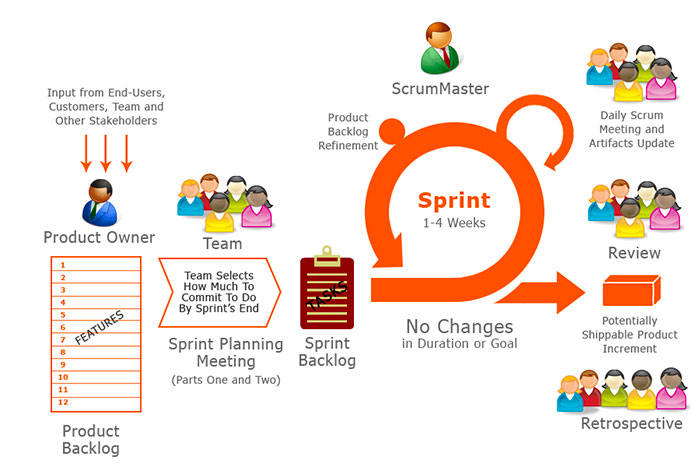
\includegraphics[scale=0.35]{immagini/scrum}
	\caption{Schema Scrum}
\end{figure}

Il team aziendale viene gestito secondo la metodologia \emph{\gls{Scrum}}\glsfirstoccur, framework \emph{\gls{agile}}\glsfirstoccur di sviluppo del sofware, introdotto nel 1995 da Ken Schwaber e Jeff Sutherland. Tale modello si basa sulla teoria del controllo empirico del processo la quale afferma che la conoscenza deriva da decisioni di esperienza e che la preparazione si basa su ciò che è già noto. \textit{Scrum}, dunque, prevede un approccio iterativo e incrementale per cercare di ottimizzare la prevedibilità e il controllo dei rischi. Sono tre i principi che sostengono la teoria del controllo empirico del processo:
\begin{enumerate}
	\item \textbf{Trasparenza} - i responsabili devono avere una visione degli aspetti più significativi del processo per poter monitorare il risultato del lavoro che sia conforme alle attese;
	\item \textbf{Ispezione} - il lavoro di uno \textit{sprint} deve poter essere ispezionato per rilevare variazioni indesiderate rispetto all'obiettivo;
	\item \textbf{Adattamento} - se durante un'ispezione viene riscontrato uno o più aspetti che si discostano dai limiti accettabili e il prodotto risulta inacettabile, il processo in esecuzione deve essere adattato e questo deve avvenire nel minor tempo possibile al fine di evitare ulteriori deviazioni.
\end{enumerate}
Il punto centrale dello \textit{Scrum} è dato dallo \textit{sprint}, esso può essere considerato come un progetto con la durata massima di 4 settimane nelle quali deve essere portato a termine e che, alla sua conclusione, porterà ad un incremento del prodotto. Durante uno \textit{sprint} non vengono apportate modifiche che potrebbero minarne l'esistenza del prodotto, inoltre gli obiettivi di qualità non devono diminuire mentre, l'ambito di applicazione del progetto, può essere chiarito e rinegoziato tra team di sviluppo e \textit{stakeholders}. Nel modello \textit{Scrum} i requisiti, le funzionalità, i miglioramenti e le correzioni sono ordinati all'interno del \emph{\gls{ProductBacklog}}\glsfirstoccur; esso non è mai completo, è dinamico ed evolve con il prodotto.\\
Lo \emph{\gls{SprintBacklog}}\glsfirstoccur, invece, è una previsione redatta in sede di riunione dal team di sviluppo con gli obiettivi che deve raggiungere lo \textit{sprint} e il lavoro che ne deriva anche in termini di tempo.\\
Lo \gls{SprintBacklog} aiuta, quindi, a rendere trasparente il lavoro necessario per raggiungere gli obiettivi dello \textit{sprint}.
Athesys adotta \textit{sprint} di durata quindicinale, preceduti da riunioni per defnire gli obiettivi e i tempi dello \textit{sprint} tra i membri del team di sviluppo. Ad ogni \textit{sprint} ne segue la sua ispezione e in caso l'adattamento con miglioramenti e correzioni.

%**************************************************************
\section{Il progetto proposto}
Il progetto nasce nel contesto di migliorare e far evolvere il sistema di \emph{\gls{IAM}}\glsfirstoccur già in utilizzo da parte dell'azienda.\\
Nelle sezioni seguenti si andrà quindi a discutere dettagliatamente il problema che si è voluto affrontare, le soluzioni che si sono trovate, l'ambito di sviluppo del prodotto, le funzionalità richieste e la pianificazione del progetto aziendale.

\subsection{Il contesto}
I servizi di identità decentralizzati permettono alle persone di registrarsi, a specifici servizi, come utenti in modo autonomo utilizzando gli \emph{\gls{identityWallet}}\glsfirstoccur. 
Da questi gli utenti possono scegliere quali attributi, del loro profilo, immagazzinare e condividere con il \textit{service provider} verso la quale si vogliono autenticare.
Nella forma più semplice l'identità è formata da due chiavi crittografiche, una pubblica ed una privata.
La chiave privata è mantenuta protetta all'interno dell'\gls{identityWallet} mentre, quella pubblica, è crittografata tramite \textit{hash} e mantenuta immutabile all'interno dell'\gls{ITF}. 
La chiave privata viene utilizzata per crittografare le informazioni e gli attributi degli utenti mentre, quella pubblica, viene utilizzata per decriptare le informazioni appena criptate. Questo meccanismo nasce allo scopo di assicurare che le informazioni, criptate, che arrivano al \textit{service provider}, appartengano all'utente che effettivamente ha richiesto l'accesso al servizio. Questo sicurezza viene garantita proprio dal meccanismo delle chiavi in quanto solo l'utente stesso può conoscere la propria chiave privata e quindi criptare le proprie informazioni.\\
Le operazioni che avvengono, sia da parte dell'utente che del \textit{service provider}, per poter permettere l'accesso ad un servizio sono le seguenti:
\begin{enumerate}
	\item l'utente via la richiesta d'accesso al \textit{service provider} inviando le proprie informazioni criptate con la sua chiave privata;
	\item il \textit{service provider} riceve le informazioni dell'utente ed un suo identificativo;
	\item il \textit{service provider} interroga l'\gls{ITF} per recuperare la chiave pubblica associata a quell'utente;
	\item il \textit{service provider} decripta le informazioni dell'utente utilizzando la chiave pubblica recuperata;
\end{enumerate}
A questo punto il \textit{service provider} è sicuro che le informazioni che ha ricevuto sono di proprietà dell'utente e può permettere o meno l'accesso al servizio richiesto.\\
Questi passaggi sono la base di due modelli di autenticazione:
\begin{itemize}
	\item Modello Centralizzato;
	\item Modello Decentralizzato;
	\item Modello basato sugli Identity Custodians.
\end{itemize}

\subsubsection{Modello Centralizzato}
\begin{figure}[!h]
	\centering
	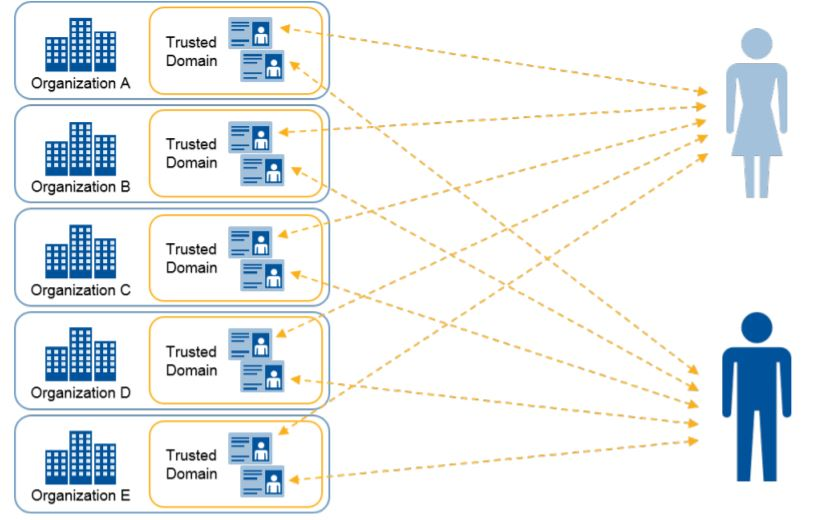
\includegraphics[scale=0.5]{immagini/ITF_Centralizzato}
	\caption{Modello Centralizzato}
\end{figure}
In un modello centralizzato, le organizzazioni stabiliscono una relazione di fiducia \textit{punti a punto} con ogni utente che interagisce con il sistema.
Le organizzazioni devono, quindi, mantenere la fiducia verso i loro utenti andando a gestire le varie identità digitali. Questo fa sì che, le organizzazioni, investano sulla protezione delle identità e delle informazioni sensibili. Questo si ripercuote, inevitabilmente, su un aumento dei costi operativi.\\
Dal lato utente, questi, non hanno alcun controllo sulla gestione delle proprie identità ed attributi.\\
Ogni organizzazione deve verificare l'identità di ogni utente prima di permettere la registrazione e l'accesso ai suoi servizi. Questo può ripetersi molte volte per, singolo utente, a seconda di quale organizzazione, l'utente, va a richiedere un servizio e a seconda del tipo di servizio che è richiesto. 
Questo modello ha fatto sì che nascesse una proliferazione di identità digitali diverse associate agli stessi utenti\cite{ITF_gartner}.
\subsubsection{Modello Decentralizzato}
\begin{figure}[!h]
	\centering
	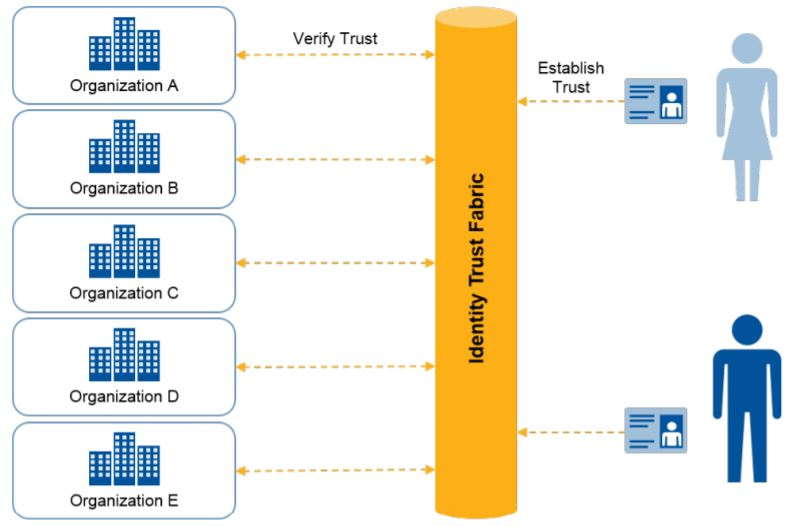
\includegraphics[scale=0.50]{immagini/ITF_Decentralizzato}
	\caption{Modello Decentralizzato}
\end{figure}
In un modello decentralizzato abbiamo un'entità terza che attesta e certifica la validità di un'identità auto-generata.
Questo tipo di modello non elimina il processo di identity proofing ma lo trasforma in un processo generalizzato che può essere utilizzato tra organizzazioni diverse.
Una volta che un'identità decentralizzata è stata legalmente provata, può essere utilizzata da service providers multipli per garantire l'accesso ai loro servizi.
Per far funzionare questo modello abbiamo bisogno di una "struttura" che immagazzini immutabilmente le informazioni ed i certificati crittografati.  Per fare questo, la \textit{Blockchain} è la tecnologia adatta.
I sistemi decentralizzati alleviano, le organizzazioni, dell'incarico di mantenere informazioni sensibili riguardo l'identità con la conseguenza di abbassare i costi di mantenimento e di gestione dei rischi.
Dal lato utente invece abbiamo un controllo maggiore sulla privacy in quanto, i sistemi decentralizzati, permettono una miglior gestione delle identità personali e dei dati.
Tuttavia la gestione completa delle informazioni personali, da parte dei singoli utenti, può risultare difficoltosa. È per questo che si è pensato di passare da un modello totalmente decentralizzato ad un modello ibrido dove le informazioni personali son custodite dagli \textit{Identity Custiodians}\cite{ITF_gartner}.
\subsubsection{Modello basato sugli Identity Custodians}
Gli \textit{Identity Custodians} nascono con l'obiettivo di semplificare la gestione e accrescere la disponibilità e protezione delle identità decentralizzate mantenendo, al loro interno, tutti gli attributi di identità necessari.
Sorgono spontanee alcune preoccupazioni in quanto, un \textit{Identity Custodian}, rimane suscettibile ad attacchi esterni in quanto mantiene informazioni sensibili e di valore nonostante siano criptate. Questo è il motivo alla base della creazione di consorzi che adempiono al compito di \textit{Identity Custodians} sfruttando la \textit{BlockChian} come tecnologia di decentralizzazione delle informazioni.\\
Utilizzato gli \textit{Identity Custodians} all'interno di un modello a consorzi si aumenta la privacy e la sicurezza delle informazioni. I dati utente ed i riferimenti ai loro hash nell'\gls{ITF} sono criptati e immagazzinati all'interno dell'ambiente decentralizzato. Questo permette all'\gls{identityWallet} di condividere solamente il riferimento alla locazione nell' \textit{Identity Custodian} facendo sì che i \textit{service provider} possano recuperare le informazioni e verificare l'identità utente prima dell'accesso\cite{ITF_gartner}.
\begin{figure}[h]
	\centering
	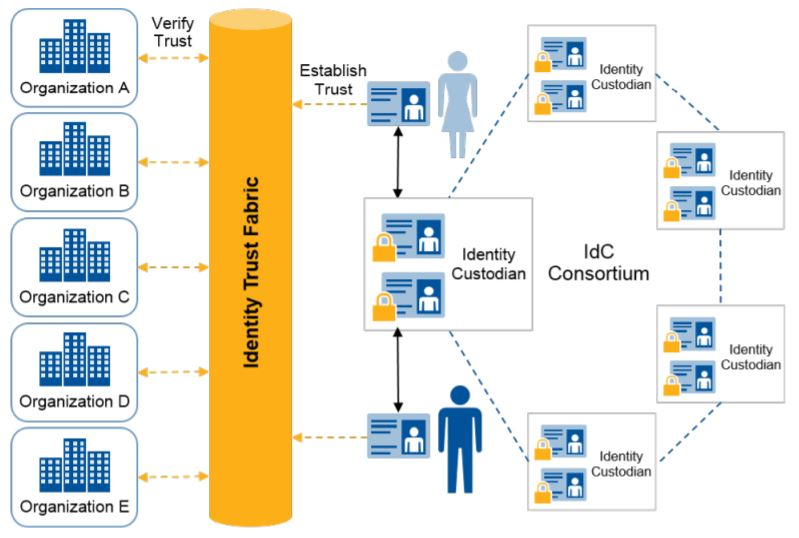
\includegraphics[scale=0.50]{immagini/ITF_IdentityCustodians}
	\caption{Modello basato sugli Identity Custodians}
\end{figure}

\subsection{Il progetto da realizzare}
Nell'ottica di estendere le funzionalità di \emph{\gls{monokee}}\glsfirstoccur, è stato previsto lo sviluppo di un layer di sicurezza, denominato \gls{ITF} (ITF), per integrare una tecnologia \textit{Blockchain} nei processi di accesso ai servizi e condivisione degli attributi di profilo.
\begin{figure}[!h]
	\centering
	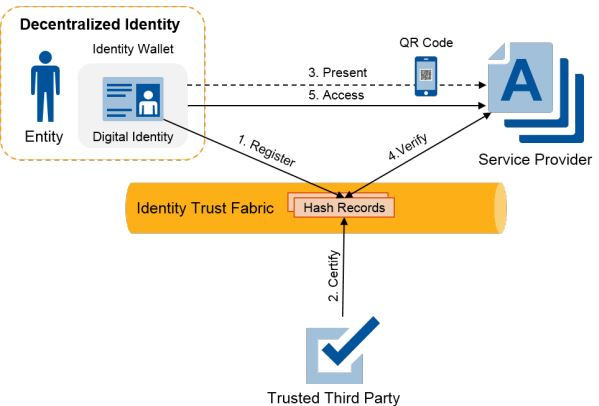
\includegraphics[scale=0.50]{immagini/ITF_Modello_Funzionale}
	\caption{Esempio di modello decentralizzato che sfrutta ITF}
\end{figure}
\\
L'immagine raffigura un tipico scenario di accesso ai servizi di un \textit{service provider} da parte di un utente che possiede un proprio \gls{identityWallet}.
Il modulo realizzato rappresenta il layer di sicurezza che si interpone tra l'utente e i servizi offerti dal \textit{service provider}.
Le funzionalità principali realizzate, come si può vedere dalla figura, son essenzialmente cinque:
\begin{enumerate}
	\item \textbf{Registrazione}: come prima cosa l'utente genera la coppia di chiavi (privata e pubblica) nell'\gls{identityWallet}. La chiave pubblica viene crittografata tramite una funzione \textit{hash one-way} (ovvero calcolare l'hash è, computazionalmente semplice, ma, partendo dall'hash, ricalcolare il valore originale è computazionalmente impossibile) e immagazzinata all'interno dell'\gls{ITF}. Al record, contenente l'identità, possono essere aggiunti ulteriori dati personali per rafforzare ancora di più il processo di \emph{\gls{identityProofing}}\glsfirstoccur e \emph{\gls{identityBinding}}\glsfirstoccur delle informazioni con l'identità digitale;
	 
	\item \textbf{Certificazione}: come parte del processo di \gls{identityProofing} una parte terza fidata ha il compito di validare l'identità dell'utente. Questa validazione può avvenire o durante il processo di \gls{identityBinding} delle informazioni con l'identità digitale o durante la fase di registrazione/accesso di un utente ad un particolare servizio. Dopo aver validato con successo le informazioni di identità, questa parte terza certifica l'identità o gli attributi dell'utente, "firmandole" con la propria chiave privata. A questo punto il record certificato viene inserito nel \gls{ITF}.
	Il processo di registrazione/autenticazione può esser semplificato se esistono già dei record, interni all'\gls{ITF}, che contengono informazioni e attributi utili. 
	Su richiesta dell'utente, le organizzazioni possono ricertificare dei record per aumentare il livello di sicurezza delle informazioni contenute senza che l'utente debba registrarsi nuovamente generando un nuovo record con le stesse informazioni. Questo viene detto \textit{Web of Trust};
	 
	\item \textbf{Presentazione}: la chiave pubblica ed il riferimento alla locazione del \textit{hash} nel \gls{ITF} vengono forniti al \textit{service provide} affinché vengano verificati prima di permettere l'accesso al servizio;
	
	\item \textbf{Verifica}: una volta che il \textit{service provider} possiede la chiave pubblica e la locazione dell'\textit{hash} nell'\gls{ITF} passa alla fase di verifica.
	In questa fase, utilizzando queste informazioni, verifica l'identità o gli attributi utente andando a generare l'\textit{hash} dei dati e, successivamente, confrontandolo con il loro corrispettivo interno all'\gls{ITF};
	 
	\item \textbf{Accesso}: dopo aver verificato con successo l'identità di un utente viene concesso, a quest'ultimo, di accedere ai servizi o alle applicazioni richieste.
\end{enumerate}
\subsection{Obiettivi di stage}
Nella seguente tabella sono riportati gli obiettivi fissati per lo stage con rispettivo identificativo, importanza e breve descrizione.\\\\
L'identificativo (abbreviato in ID) userà la notazione:\\
\centerline{[\textit{Importanza}][\textit{numero identificativo}]}.\\
L'importanza sarà rappresentata da una delle seguenti lettere maiuscole:\\
\centerline{\textbf{O},\textbf{D},\textbf{F}}\\
che identificano, rispettivamente, un obiettivo obbligatorio, desiderabile o facoltativo.\\
Il numero idetificativo è un numero incrementale che segnala in modo univoco l’obiettivo.\\
L'importanza di un obiettivo viene assegnata come segue:
\begin{itemize}
	\item \textbf{Obbligatorio} - rappresenta un requisito che dovrà esser soddisfatto al fine di garantire le funzionalità base del sistema;
	\item \textbf{Desiderabile} - rappresenta un requisito il cui non soddisfacimento non pregiudica le funzionalità base ma, la sua realizzazione, da un valore aggiunto importante al fine di realizzare un sistema più completo;
	\item \textbf{Facoltativo} - rappresenta un requisito che, se soddisfatto, renderebbe il sistema ancora più completo a discapito di un uso di risorse.
\end{itemize}
\begin{longtable}{|r l|p{3cm}|p{10cm}|}
	\hline
	\multicolumn{2}{|c|}{\textbf{ID}} & \textbf{IMPORTANZA} & \textbf{DESCRIZIONE}\tabularnewline
	\hline
	& O1 & Obbligatorio & Studio del dominio applicativo \\\hline
	& O2 & Obbligatorio & Studio delle possibili tecnologie \textit{Blockchain} da adottare \\\hline
	& O3 & Obbligatorio & Analisi comparativa delle tecnologie \textit{Blockchain} individuate \\\hline
	& O4 & Obbligatorio & Definizione dei vari casi d'uso per le funzionalità richieste (sopracitate) \\\hline
	& O4.1 & Obbligatorio & Definizione dei casi d'uso per la funzionalità di registrazione \\\hline
	& O4.2 & Obbligatorio & Definizione dei casi d'uso per a funzionalità di certificazione \\\hline
	& O4.3 & Obbligatorio & Definizione dei casi d'uso per la funzionalità di verifica \\\hline
	& O5 & Obbligatorio & Stesura del documento di analisi dei requisiti\\\hline
	& O6 & Obbligatorio & Stesura del documento contenete le specifiche architetturali del sistema \\\hline
	& O7 & Obbligatorio & Realizzazione del modulo \gls{ITF}\\\hline
	& O7.1 & Obbligatorio & Realizzazione della struttura e della gerarchia di classi necessaria alla realizzazione del modulo \\\hline
	& O7.2 & Obbligatorio & Implementazione dei metodi necessari per il corretto funzionamento del modulo\\\hline
	& D1 & Desiderabile & Produzione della documentazione relativa alle analisi svolte \\\hline
	& D2 & Desiderabile & Definizione dei casi d'uso per la funzionalità di presentazione dei dati \\\hline
	& D3 & Desiderabile & Definizione dei casi d'uso per la funzionalità di accesso al servizio \\\hline
	& D4 & Desiderabile & Stesura del documento di progettazione\\\hline
	& D5 & Desiderabile & Realizzazione dei test necessari alla verifica del corretto funzionamento del sistema\\\hline
	& D5.1 & Desiderabile & Implementazione dei test di unità per i singoli metodi\\\hline
	& D5.2 & Desiderabile & Implemetnazione dei test di integrazione per testare le classi \\\hline
	& D5.3 & Desiderabile & Implementazione dei test di integrazione per testare l'interazione tra tutte le classi che compongono il sistema \\\hline
	& F1 & Facoltativo & Stesura del documento relativo ai test di unità ed integrazione \\\hline	
	& F2 & Facoltativo & Stesura del documento relativo alla validazione del modulo (anomalie e bug) \\\hline
	\caption{Tabella degli obiettivi di stage}
\end{longtable}
\subsection{Pianificazione del lavoro}
In accordo con l'azienda tutto il periodo di stage che va dal 4 Giugno 2018 al 30 Luglio 2018 è stato suddiviso in fasi.\\
Vengono qui riportate in dettaglio le attività previste per ogni periodo, specificando il numero di ore preventivate e il periodo in cui ne è stato pianificato lo svolgimento.\\\\
\subsubsection{Fase 1: dal 4 Giugno 2018 all'8 Giugno 2018 per un totale di 40 ore}
In questa prima fase si era prevista l'individuazione della tecnologia \textit{Blockchain} da adottare per l'implementazione del modulo \gls{ITF}. La scelta della tecnologia prevedeva l'analisi ed il confronto delle varie tecnologie candidate in rapporto al dominio applicativo ovvero la gestione delle identità e degli accessi ai servizi.\\
In questa prima fase era prevista la stesura del documento di studio di Fattibilità.\\\\

\subsubsection{Fase 2: dall' 11 Giugno 2018 al 15 Giugno 2018 per un totale di 40 ore}
In questa fase, lo scopo principale era studiare approfonditamente il sistema che si voleva realizzare e definire tutti i casi d'uso necessari per modellare, concettualmente, l'interno sistema.\\
Il mio stage, essendo fatto in collaborazione con un altro studente, prevedeva l'individuazione dei casi d'uso relativi alle funzionalità di:
\begin{itemize}
	\item Registrazione;
	\item Certificazione;
	\item Verifica.
\end{itemize}
Di cui si è discusso precedentemente.\\
Questa fase prevedeva la stesura del documento di Analisi dei Requisiti.\\\\

\subsubsection{Fase 3: dal 18 Giugno 2018 al 22 Giugno 2018 per un totale di 40 ore}
In questa terza fase era prevista la stesura dell'architettura generale, comprensiva di \emph{\gls{designPatterns}}\glsfirstoccur, che avrebbe implementato le funzionalità rilevate dai casi d'uso della fase precedente.\\
Si era previsto anche la stesura del documenti di Progettazione Architetturale.\\\\

\subsubsection{Fase 4: dal 25 Giugno 2018 al 4 Luglio 2018 per un totale di 60 ore}
Quarta fase del periodo di stage che prevedeva la definizione dei metodi, necessari per l'implementazione del sistema, in pseudo-codice. Anche in questa fase era prevista la stesura di un documento, desiderabile, di Progettazione di Dettaglio.\\\\

\subsubsection{Fase 5: dal 5 Luglio 2018 al 25 Luglio 2018 per un totale di 120 ore}
Fase centrale di tutto lo stage in cui era prevista la codifica del modulo \gls{ITF} comprensiva di classi e metodi.\\
Sempre durante questa fase era prevista anche la codifica dei test di unità e di integrazione per i singoli metodi e per le classi.\\
A corredo di tutto questo era prevista la stesura del documento relativo al testing delle funzionalità.\\\\

\subsubsection{Fase 6: dal 26 Luglio 2018 al 30 Luglio 2018 per un totale di 20 ore}
In quest'ultima fase era prevista la validazione dell'intero sistema realizzato e predisposto il software per il collaudo finale fatto in collaborazione con l'altro studente stagista che ha realizzato le componenti mancanti per l'implementazione del modulo \gls{ITF} finale.\\\\

Al termine di questo periodo di stage il prodotto si trova in una fase di \emph{\gls{poc}}\glsfirstoccur funzionante e predisposta per:
\begin{itemize}
	\item poter implementare nuove future funzionalità;
	\item migliorare le funzionalità che già possiede senza dover apportare grossi cambiamenti all'infrastruttura;
	\item poter essere integrato come parte del prodotto cardine dell'azienda: \gls{monokee}.
\end{itemize}

\subsubsection{Riepilogo delle attività previste}
\begin{longtable}{|r l|p{1cm}|p{3cm}|}
	\hline
	\multicolumn{2}{|c|}{\textbf{ATTIVITÀ}} & \textbf{ORE} & \textbf{PERIODO}\tabularnewline
	\hline
	& Fase 1 & 40 & 08/06 - 22/06 \\\hline	
	& Fase 2 & 40 & 11/06 - 15/06\\\hline
	& Fase 3 & 40 & 18/06 - 22/06\\\hline
	& Fase 4 & 60 & 25/06 - 04/07 \\\hline
	& Fase 5 & 120 & 05/07 - 25/07 \\\hline
	& Fase 6 & 20 & 26/07 - 30/07 \\\hline	
	\caption{Riepilogo delle attività di stage}
\end{longtable}
%**************************************************************
